\documentclass[11pt,a4paper]{article}
\usepackage[margin=2.2cm]{geometry}
\usepackage{booktabs}
\usepackage{graphicx}
\usepackage{amsmath}
\usepackage{float}
\usepackage[hidelinks]{hyperref}

\title{Assignment 2: Attention Mechanisms and Transformers}
\author{}
\date{}

\begin{document}
\maketitle
\vspace{-1.5cm}

\section{Part A: Self-Attention From Scratch}

We implemented scaled dot-product self-attention for the sentence \texttt{"Darth Vader is the villain"} (5 tokens). Each token was assigned a random 4-dimensional embedding, and three fixed (untrained) weight matrices $W_Q, W_K, W_V \in \mathbb{R}^{4 \times 3}$ projected them into query, key, and value vectors. Attention was computed as $\text{Attention}(Q,K,V) = \text{softmax}(QK^\top / \sqrt{d_k})\, V$ with $d_k = 3$.

\begin{table}[H]
\centering
\begin{tabular}{l|ccccc}
\toprule
         & Darth & Vader & is    & the   & villain \\
\midrule
Darth    & 0.135 & 0.050 & 0.291 & 0.169 & 0.356 \\
Vader    & 0.051 & 0.309 & 0.249 & 0.285 & 0.106 \\
is       & 0.324 & 0.055 & 0.206 & 0.119 & 0.296 \\
the      & 0.192 & 0.167 & 0.229 & 0.201 & 0.210 \\
villain  & 0.142 & 0.388 & 0.144 & 0.208 & 0.118 \\
\bottomrule
\end{tabular}
\caption{Self-attention weights (rows = queries, columns = keys). Each row sums to 1.}
\end{table}

Since the projection matrices are random and untrained, the attention weights do not reflect semantic relationships. However, the mechanism is correct: each token's context vector is a weighted combination of all value vectors, where weights are determined by query--key compatibility. In a trained model, semantically related pairs like ``villain'' and ``Vader'' would receive high attention weights. Interestingly, ``villain'' already attends most strongly to ``Vader'' (0.388) purely by chance in this random initialisation.

\begin{figure}[H]
    \centering
    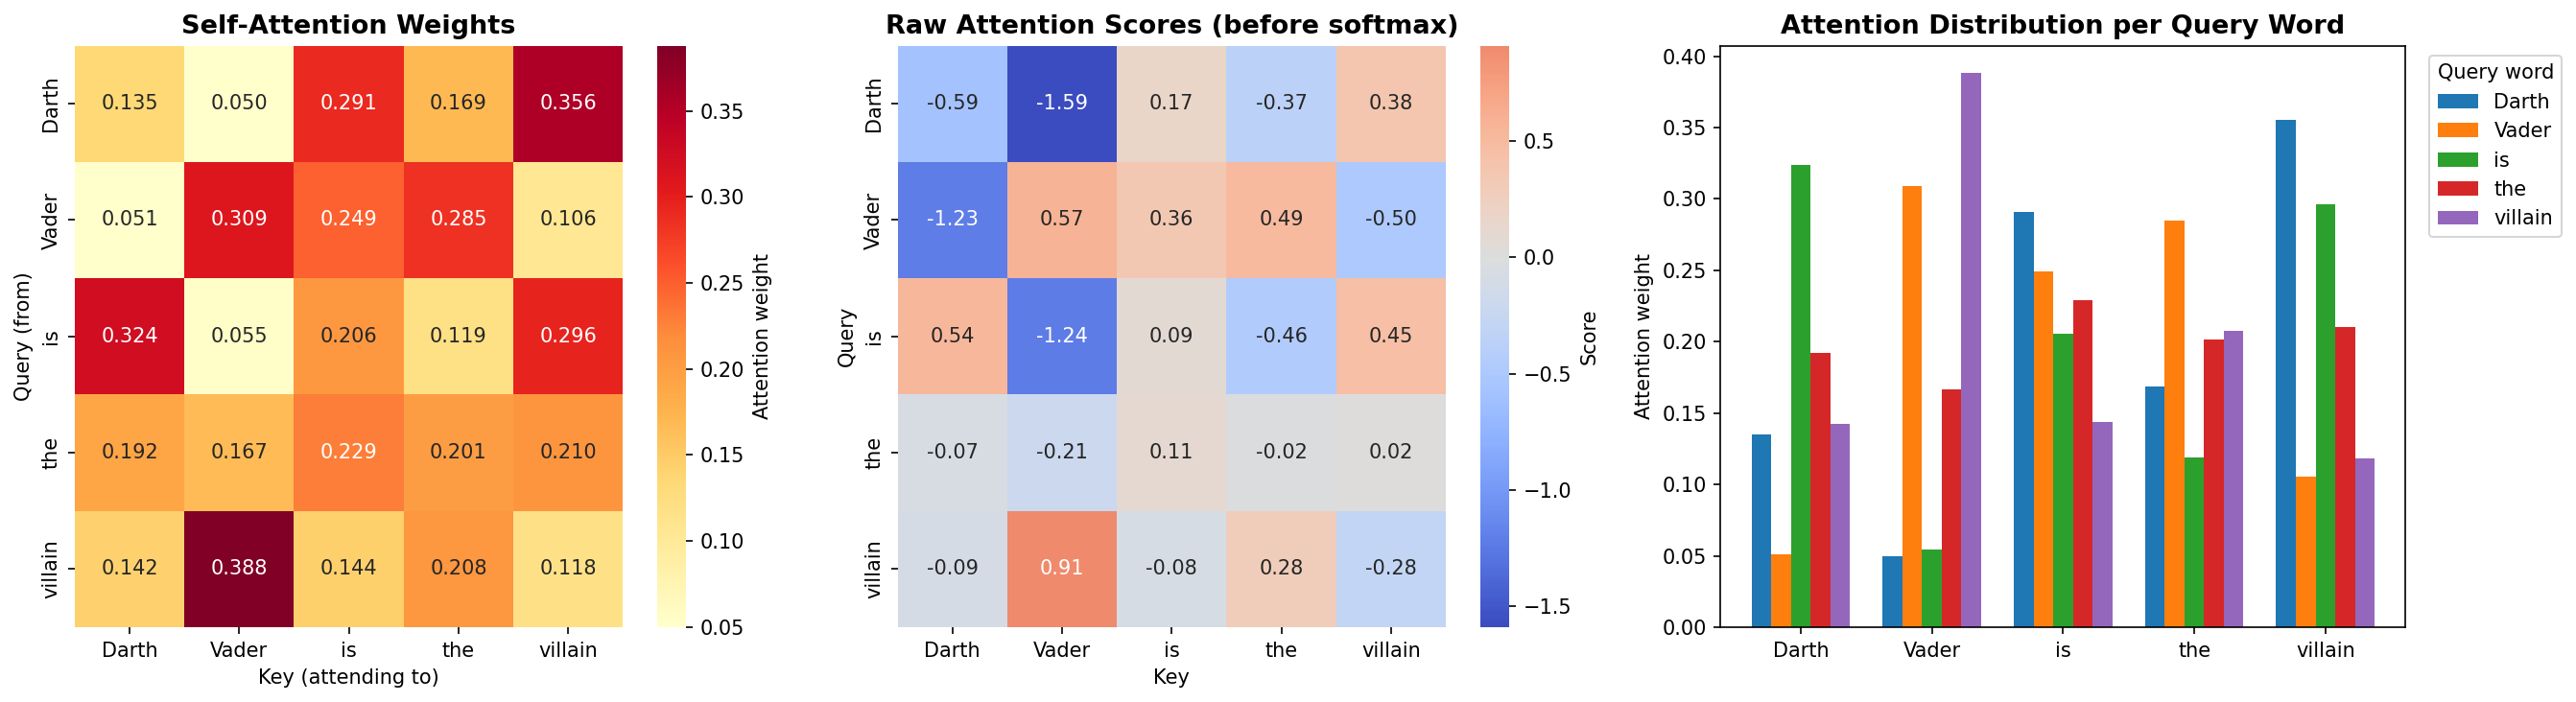
\includegraphics[width=\textwidth]{attention_visualisation.png}
    \caption{Left: attention weight heatmap. Centre: raw scores before softmax. Right: per-query attention distribution.}
\end{figure}

\section{Part B: Transformer-Based Movie Chatbot}

We used T5-small (60.5M parameters), a pretrained encoder-decoder Transformer, to build a simple movie QA chatbot. A small corpus of 6 movies (Star Wars, The Godfather, The Dark Knight, Inception, Titanic, Pulp Fiction) with IMDb-style plot summaries was prepared, yielding 24 QA pairs. Each input follows the format \texttt{question: ... context: ...}, and the model generates the answer as free text. Fine-tuning was intentionally minimal: 3 epochs with AdamW ($lr = 3 \times 10^{-4}$, batch size 4). The loss decreased from 0.592 to 0.303 but remained high, confirming the model did not converge.

\begin{table}[H]
\centering
\begin{tabular}{p{6.5cm}p{4cm}c}
\toprule
\textbf{Question} & \textbf{Model Answer} & \textbf{Correct?} \\
\midrule
Who is the villain in Star Wars? & Christian Bale & $\times$ \\
What movie features Darth Vader? & The Galactic Empire & $\times$ \\
Who directed The Godfather? & Francis Ford Coppola & $\checkmark$ \\
Who plays the Joker in The Dark Knight? & Christian Bale & $\times$ \\
What happens to the Titanic? & It hits an iceberg and sinks & $\checkmark$ \\
Who stars in Inception? & Christian Bale & $\times$ \\
Who directed Pulp Fiction? & Quentin Tarantino & $\checkmark$ \\
Who is the villain in Titanic? & Christian Bale & $\times$ \\
What year was Inception released? & 2010 & $\checkmark$ \\
Who plays Mia Wallace in Pulp Fiction? & Uma Thurman & $\checkmark$ \\
\bottomrule
\end{tabular}
\caption{Chatbot test results (5/10 correct).}
\end{table}

The model achieved 50\% accuracy. It answers factual questions well (directors, years, plot events) but shows a strong ``default answer'' bias toward ``Christian Bale,'' suggesting it latched onto a frequent name during fine-tuning rather than learning the QA mapping properly.

\section{Analysis}

\textbf{Failures and hallucination.} The model hallucinates confidently: it answers ``Christian Bale'' for Star Wars, Inception, and Titanic---movies where Bale does not appear. This is a direct consequence of minimal fine-tuning on only 24 examples over 3 epochs. The model also struggles with answer-type disambiguation (returning ``The Galactic Empire'' instead of a movie title) and with questions that have no answer in the corpus (``Who is the villain in Titanic?'').

\textbf{How attention helps in long contexts.} Self-attention allows every token to attend directly to every other token regardless of distance. This means the model can link ``villain'' in the question to ``Darth Vader'' hundreds of tokens away in the context without passing through intermediate hidden states (as RNNs must). Multi-head attention further enables different heads to capture different relationship types (syntactic, semantic, coreference) in parallel. This $O(1)$ path length between any two positions is the fundamental advantage over recurrence ($O(n)$ steps) and convolution ($O(\log n)$ layers).

\textbf{Dataset vs.\ model limitations.} On the dataset side: the corpus is tiny (6 movies, 24 QA pairs), each question phrasing is seen only once, and some queries have no answer in the text. On the model side: T5-small has limited capacity, 512-token input truncation cuts off part of the concatenated context, and 3 epochs of fine-tuning is insufficient to learn the task. With more data, more diverse question phrasings, and more training epochs, accuracy would improve substantially---but even with this minimal setup, the model demonstrates that pretrained Transformers can extract and generate answers from unstructured text.

\end{document}
